%% Exercice 3

%\ExoSpecs{\TTBF{CalculTVA.sh}}{\TTBF{\RenduDir/src/exo1/}}{750}{640}{\TTBF{write}}
\ExoSpecsCustom{\TTBF{bt\_bst.c}}{\TTBF{\RenduDir/src/}}{750}{640}{Fonctions autorisées}{\TTBF{malloc(3)}, \TTBF{free(3)}, \TTBF{printf(3)}}

\vspace*{0.7cm}

\noindent \ExoObjectif{Le but de l'exercice est d'implémenter une mini bibliothèque d'arbres binaires de recherche (ABR).}

\bigskip

%\noindent Les fonctions demandées dans cet exercice devront se trouver dans une bibliothèque nommée \TTBF{libmystack}.
%Après un appel à la commande \texttt{make} à la racine du projet, il faut que votre chaîne de compilation produise à la racine de votre projet une version statique de la bibliothèque (qui se nommera \TTBF{libmystack.a}) ainsi qu'une version dynamique de la bibliothèque (qui se nommera \TTBF{libmystack.so}).
%
%\bigskip

\noindent Vous devez écrire plusieurs fonctions permettant d'effectuer des recherche, insertions, et suppressions de nœuds dans des ABR.
Un fichier \TTBF{bt\_bst.h} contenant toutes les fonctions exportables à implémenter vous est fourni en annexe.
Celui-ci s'appuie sur le fichier \TTBF{bt\_basics.h} de l'exercice 1 : vous devez avoir réalisé toutes les fonctions du premier exercice pour pouvoir faire celui-ci.


\bigskip

%\noindent Conceptuellement, les fonctions manipulant des piles de type \TTBF{stack\_ll*} devront pouvoir gérer ces 3 cas :

%\bigskip

%\begin{center}
%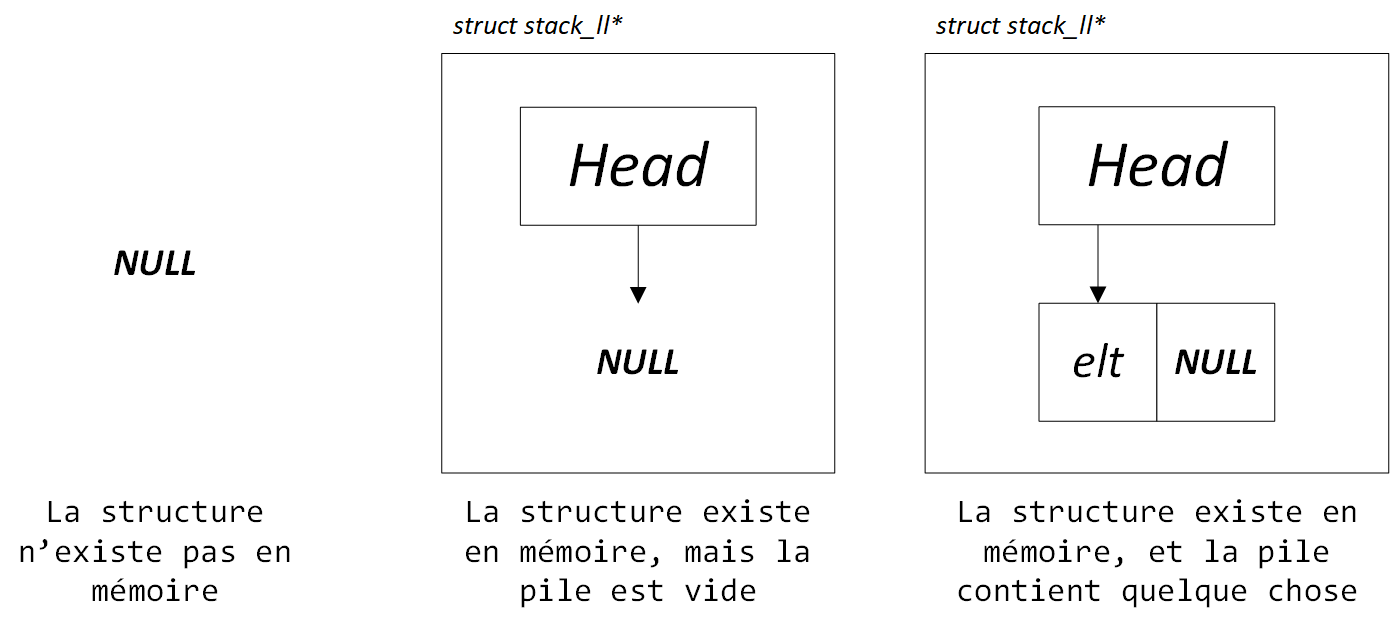
\includegraphics[scale=0.85]{Cours/Piles_Implementation_LL.png}
%\end{center}

\bigskip
%\newpage

\noindent Vous devez implémenter les fonctions suivantes :

\bigskip

\lstset{language=C}
%\begin{lstlisting}[frame=single,title={Liste des fonctions pour une pile avec liste chaînée}]
\begin{lstlisting}[frame=single]
bt_p *search_bt_p(bt_p *T, int key);
bt_p *search_verbose_bt_p(bt_p *T, int key);

bt_p *insert_leaf_bt_p(bt_p *T,
                       int key,
                       int len_elt,
                       void *elt);

bt_p *remove_node_bt_p(bt_p *T, int key);

bt_t *convert_bt_p_to_tab(bt_p *T);
void print_bt_t(bt_t *T_tab);

bt_p *insert_root_rot_bt_p(bt_p *T
                           int key,
                           int len_elt,
                           void *elt);

bt_p *insert_root_cut_bt_p(bt_p *T       // BONUS
                           int key,
                           int len_elt,
                           void *elt);
\end{lstlisting}


\subsubsection*{\TTBF{bt\_p *search\_bt\_p(bt\_p *T, int key)}}

\noindent Cette fonction recherche un nœud à partir de sa clé dans un arbre binaire en appliquant les contraintes des ABR.
Si la clé est trouvée, on renvoie un pointeur vers le nœud contenant la clé.
Si la clé n'est pas trouvée, ou que le l'arbre binaire est \TTBF{NULL}, alors la fonction doit renvoyer un pointeur \TTBF{NULL}.

\bigskip


\subsubsection*{\TTBF{bt\_p *search\_verbose\_bt\_p(bt\_p *T, int key)}}

\noindent Cette fonction recherche un nœud à partir de sa clé dans un arbre binaire en appliquant les contraintes des ABR et en affichant la clé de chaque nœud traversé.
Lors du parcours, chaque nœud testé verra sa clé affichée et suivie d'un retour à la ligne.
Si le nœud testé n'existe pas, il n'affichera rien (ni retour à la ligne, ni erreur).
Si la clé est trouvée, on renvoie un pointeur vers le nœud contenant la clé.
Si la clé n'est pas trouvée, ou que le l'arbre binaire est \TTBF{NULL}, alors la fonction doit renvoyer un pointeur \TTBF{NULL}.

\noindent Le format attendu est le suivant :

\bigskip

\noindent \TTBF{\textit{clé}\textbackslash{}n}

\bigskip

\noindent Ce qui donnerait ces affichages pour l'arbre suivant :

\begin{table}[ht!]
  \centering
  \begin{minipage}{0.45\textwidth}
    \centering

\lstset{language=sh}
\begin{lstlisting}[frame=single]
$ ./bt_example3 24
42
21
24
$
\end{lstlisting}

  \end{minipage}
  \hfillx
  \begin{minipage}{0.45\textwidth}
    \centering

%  level/.style = {sibling distance = 30mm/#1},
%  level 3/.style={sibling distance = 9mm},
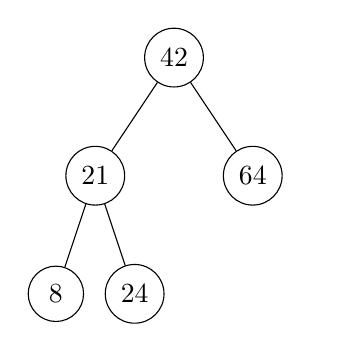
\begin{tikzpicture}[
  level/.style = {sibling distance = 20mm/#1},
  every node/.style = {minimum width = 2em, draw, circle},
  ]
  \node (n42) {42}
  child { node (n21) {21}
          child { node (n8)  {8}  }
          child { node (n24) {24} }
        }
  child { node (n64) {64}
          child { node [draw=none] (n48) {\phantom{48}} edge from parent [draw=none] }
          child { node [draw=none] (n72) {\phantom{72}} edge from parent [draw=none] }
        };
\end{tikzpicture}

  \end{minipage}
\end{table}


\begin{table}[ht!]
  \centering
  \begin{minipage}{0.45\textwidth}
    \centering

\lstset{language=sh}
\begin{lstlisting}[frame=single]
$ ./bt_example3 96
42
64
$
\end{lstlisting}

  \end{minipage}
  \hfillx
  \begin{minipage}{0.45\textwidth}
    \centering

%  level/.style = {sibling distance = 30mm/#1},
%  level 3/.style={sibling distance = 9mm},
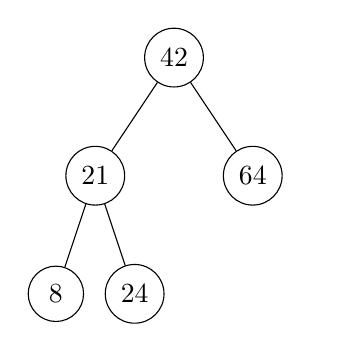
\begin{tikzpicture}[
  level/.style = {sibling distance = 20mm/#1},
  every node/.style = {minimum width = 2em, draw, circle},
  ]
  \node (n42) {42}
  child { node (n21) {21}
          child { node (n8)  {8}  }
          child { node (n24) {24} }
        }
  child { node (n64) {64}
          child { node [draw=none] (n48) {\phantom{48}} edge from parent [draw=none] }
          child { node [draw=none] (n72) {\phantom{72}} edge from parent [draw=none] }
        };
\end{tikzpicture}

  \end{minipage}
\end{table}


\subsubsection*{\TTBF{bt\_p *insert\_leaf\_bt\_p(bt\_p *T, int key, int len\_elt, void *elt)}}

\noindent Cette fonction insère un nouvel élément et sa clé dans l'arbre binaire donné en paramètre.
L'insertion doit être faite en feuille en respectant les contraintes des ABR.
La fonction doit renvoyer l'adresse de la racine.
Si l'arbre binaire en paramètre est vide, vous devez le créer et lui allouer un premier nœud qui servira de racine.
Si la clé donnée en paramètre est inférieure ou égale à $ 0 $, alors la fonction ne fera rien et renverra l'arbre inchangé.

\bigskip


\subsubsection*{\TTBF{bt\_p *remove\_node\_bt\_p(bt\_p *T, int key)}}

\noindent Cette fonction supprime un nœud de l'arbre binaire donné en paramètre à partir de la clé également donnée en paramètre.
La suppression doit être faite en respectant les contraintes des ABR.
Pour l'implémentation de cette suppression, dans le cas où le nœud visé a 2 fils, vous devrez utiliser le plus proche voisin \textit{plus petit} pour le remplacer (donc aller chercher le plus grand nœud dans le sous-arbre gauche).

\noindent Vous devez libérer correctement la mémoire en libérant le nœud, mais sans libérer l'élément stocké dans le nœud (c'est à l'utilisateur de s'en charger).
%Si l'arbre donné en paramètre est \TTBF{NULL}, la fonction doit renvoyer \TTBF{NULL}, sinon on renvoie un pointeur vers la racine.
La fonction renvoie un pointeur vers la racine de l'arbre, mais si l'arbre est vide ou le devient, la fonction renvoie \TTBF{NULL}.

%\bigskip
\medskip


\subsubsection*{\TTBF{bt\_t *convert\_bt\_p\_to\_tab(bt\_p *T)}}

\noindent Cette fonction transforme un arbre binaire au format pointeur vers le format tableau.
La structure \TTBF{bt\_t} renvoyée par la fonction contiendra :
\begin{itemize}
\item \TTBF{int tab\_len} : un champs stockant la taille des tableaux (la taille étant obligatoirement au format $ 2^{n} - 1 $ où $ n $ est le nombre de niveaux)
\item \TTBF{int tab\_used} : un champs stockant le nombre de cases utilisées dans chaque tableau (c'est-à-dire le nombre de nœuds dans l'arbre)
\item \TTBF{int *keys} : un tableau d'entiers contenant les clés des nœuds
\item \TTBF{int *elts\_size} : un tableau d'entiers contenant la taille des éléments stockés
\item \TTBF{void **elts} : un tableau de \TTBF{void*} contenant les adresses des éléments stockés (c'est-à-dire les pointeurs vers les éléments)
\end{itemize}
Les cases représentant les nœuds vides doivent contenir $ -1 $.
Si l'arbre donné en paramètre est \TTBF{NULL}, la fonction doit renvoyer \TTBF{NULL} sans rien allouer.

%\bigskip
\medskip


\subsubsection*{\TTBF{void print\_bt\_t(bt\_t *T\_tab)}}

\noindent Cette fonction affiche les clés de l'arbre binaire représenté sous forme de tableau.
Le format d'affichage est le même que pour l'affichage hiérarchique de l'exercice 1 (donc une clé par ligne, et aucun affichage si l'arbre est vide).

%\bigskip
\medskip

\subsubsection*{\TTBF{bt\_p *insert\_root\_rot\_bt\_p(bt\_p *T, int key, int len\_elt, void *elt)}}

\noindent Cette fonction insère un nouvel élément et sa clé dans l'arbre binaire donné en paramètre.
L'insertion doit être faite en racine avec la méthode des rotations.
Si l'arbre binaire en paramètre est vide, vous devez le créer et lui allouer un premier nœud qui servira de racine.
Si la clé donnée en paramètre est inférieure ou égale à $ 0 $, alors la fonction ne fera rien et renverra l'arbre inchangé.

%%\bigskip
%\medskip
%
%\subsubsection*{\textbf{[BONUS] }\TTBF{bt\_p *insert\_root\_cut\_bt\_p(bt\_p *T, int key, int len\_elt, void *elt)}}
%
%\noindent Cette fonction insère un nouvel élément et sa clé dans l'arbre binaire donné en paramètre.
%L'insertion doit être faite en racine avec la méthode de coupe.
%Si l'arbre binaire en paramètre est vide, vous devez le créer et lui allouer un premier nœud qui servira de racine.
%Si la clé donnée en paramètre est inférieure ou égale à $ 0 $, alors la fonction ne fera rien et renverra l'arbre inchangé.
